\documentclass[10pt,a4paper]{article}
\usepackage{amsmath}
\usepackage{graphicx}
\usepackage{listings}
\usepackage[margin=1in]{geometry}
\graphicspath{{./images/}}
\usepackage[backend=biber, bibencoding=utf8]{biblatex}
\addbibresource{./pres/ref.bib}

\lstset{frame=tb,
	language=R,
	basicstyle=\small,
	aboveskip=3mm,
	belowskip=3mm,
	showstringspaces=false,
	numbers=none,
	breaklines=true,
	tabsize=2,
	breakatwhitespace=true
}

\title{\vspace{-2.0cm} Bayesball \\
\large Empirical Estimation of Batting Averages
}
\date{\today}
\author{Nick Sun}

\begin{document}

\maketitle

\begin{abstract}
	Batting averages in baseball are calculated as a cumulative statistic over the course of a season, starting at zero.
	The small number of at-bats a player has per game leads to a large variance in batting average as an estimate of $p$, the true porbability of a player getting a hit in a given at-bat, especially in the early season.
	In this project, I used simulations to evaluate a Bayesian approach to estimating batting average using a Beta prior based on the previous season's performance.
	The Bayesian estimation produced an estimate of $p$ with a lower MSE than traditional batting average calculations and credible intervals that were narrower than frequentist intervals.
\end{abstract}

\section{Introduction}
No number is more important or ubiquitous in sabermetrics than batting averages, which is simply $\frac{\text{Hits}}{\text{At-bats}}$.
Batting average is calculated cumulatively over the season, starting at .000 for all players.
This makes the variance of early season batting average calculations quite large.
If we think of these batting averages as an estimation of $p$, a batter's true probability of getting a hit in an at-bat, is there a ``better'' $\hat{p}$ than traditional batting average?

\section{Methods}
One approach to estimating $p$ we can use is empirical Bayesian estimation.
If for a given player we have a prior $\pi(p) \propto p^{\alpha-1} (1 -p)^{\beta-1}$ and some data on that players hits $H$ and at-bats $AB$, then our posterior distribution will be:
\begin{align*}
\pi(p | AB, H) \propto p^{\alpha + H - 1} (1 - p)^{\beta + AB - H - 1}
\end{align*}
It is known that the mean of a beta distribution is given by $\frac{\alpha}{\alpha+\beta}$, which we can use as an estimate for $p$.

Bayesian estimation allows us to make bayesian credible intervals which we can compare against frequentist confidence intervals. 
\begin{itemize}
	\item \textbf{Bayesian Credible interval}: \texttt{qbeta(c(.025, .975), alpha0 + cumH, beta0 + cumAB - cumH)}
	\item \textbf{Jeffrey's interval}: Frequentist interval which derives from using a noninformative Beta prior $\alpha=.5, \beta=.5$: \texttt{qbeta(c(.025, .975), .5 + cumH, .5 + cumAB - cumH)}
	\item \textbf{Clopper-Pearson interval}: Another frequentist interval which is based on a binomial distribution \texttt{qbeta(.025, cumH, cumAB - cumH + 1), qbeta(.975, cumH + 1, cumAB - cumH)}
\end{itemize}
where $cumH$ and $cumAB$ are the cumulative hits and at-bats at any given point in the season.\cite{robinson}

For our simulations, we will use data from Michael Conforto (aka "Scooter") is a promising right fielder for the New York Mets.
His young career so far has been somewhat inconsistent, fluctuating between average to All-Star.\cite{baseballreference}

\begin{minipage}{.6\textwidth}
	\begin{center}
	\begin{tabular}{|| c | c | c|  c ||}
		\hline
		Season & AB & H & Batting Average \\
		\hline
		2015 & 174 & 47 & .270 \\
		2016 & 304 & 67 & .220 \\
		2017 & 373 & 104 & .279* \\
		2018 & 543 & 132 & .243 \\
		2019 & 549 & 141 & .257 \\
		\hline
	\end{tabular}
	\end{center}
\end{minipage}
\begin{minipage}{.38\textwidth}
	\begin{center}
	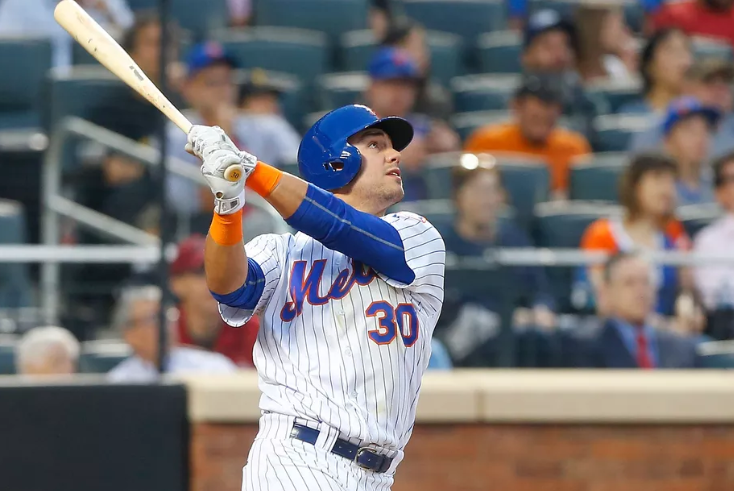
\includegraphics[width=.95\textwidth]{scooter}
	\end{center}
\end{minipage}

\subsection{Prior}

A reasonable place to start with a prior is at team level since players .
 is a density histogram of all batting averages from the 2018 New York Mets\cite{lahman} as well as an overlaid curve with MLE estimates for $\alpha$ and $\beta$.
We can try ``shifting'' the mean of this overall Mets distribution by changing the value of $\alpha$ to Michael Conforto's batting average in 2018.
While this will also change the variance of the beta prior, it is the easiest way to get an informative conjugate prior centered at last season's batting averages.

\begin{center}
	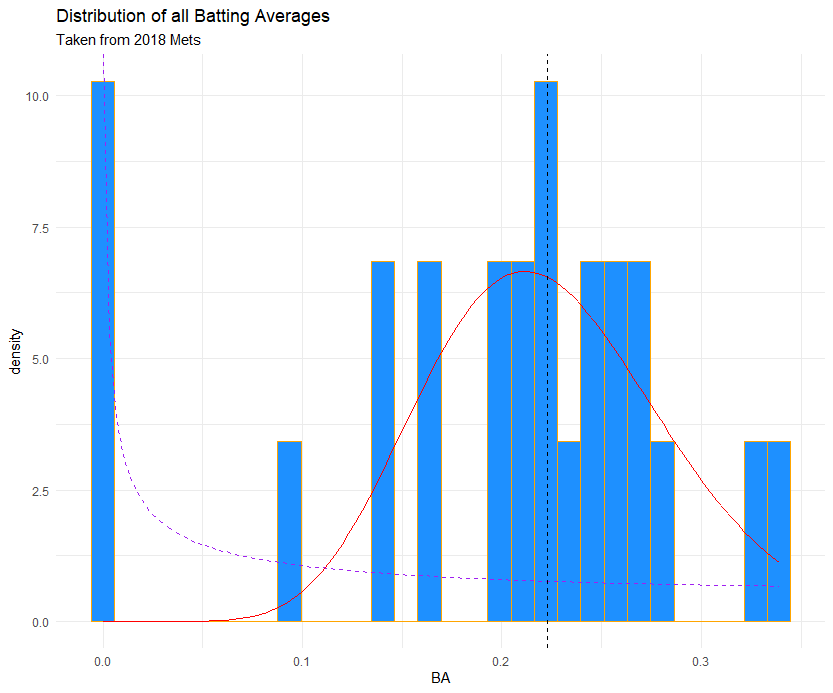
\includegraphics[width=.5\textwidth]{2018_mets_prior}
\end{center}

\section{Results}

I used three simulation scenarios with 1000 seasons apiece to compare Bayesian estimation to traditional batting average:
\begin{itemize}
	\item $p$ is a constant value over the season and is the same for every simulation
	\item $p$ is a constant value over the season, but every season has a different value
	\item $p$ changes every game, randomly sampled from a distribution
\end{itemize}

\subsection{Constant $p$ over all simulated seasons}
In 2018, Conforto had a batting average of .243 which produced a prior of Beta(11.74, 36.76) using our beta shifting technique.
Michael Conforto had a .257 batting average in 2019. If we treat this as the true value of $p$, we can simulate 1000 2019 seasons with that true value using publicly available game logs and check the MSE of our estimates at each game in the season.
MSE is calculated as the average of the squared deviations from the true value of $p$, which we can plot for both the Bayesian and frequentist estimates as the season progresses.
For each game, I also calculated the proportion in which $p$ fell within each of the three intervals.
Also displayed are the confidence and credible intervals over the course of the season.

\begin{figure}[ht]
	\centering
	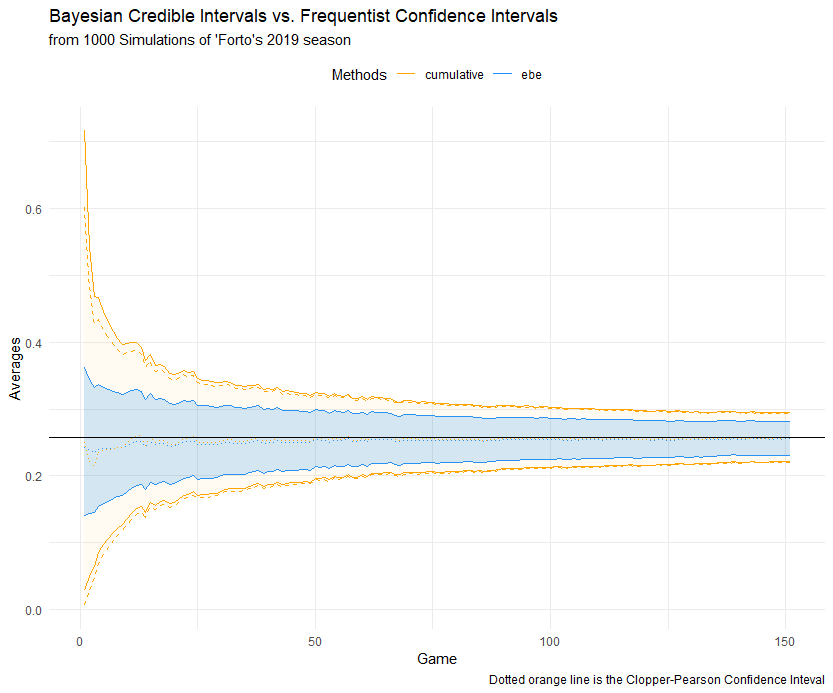
\includegraphics[width=.7\linewidth]{intervals_2019}
	\caption{\label{fig:intervals_2019} Median confidence and credible intervals for all 1000 simulated seasons shown here}
\end{figure}

\begin{minipage}{.5\textwidth}
	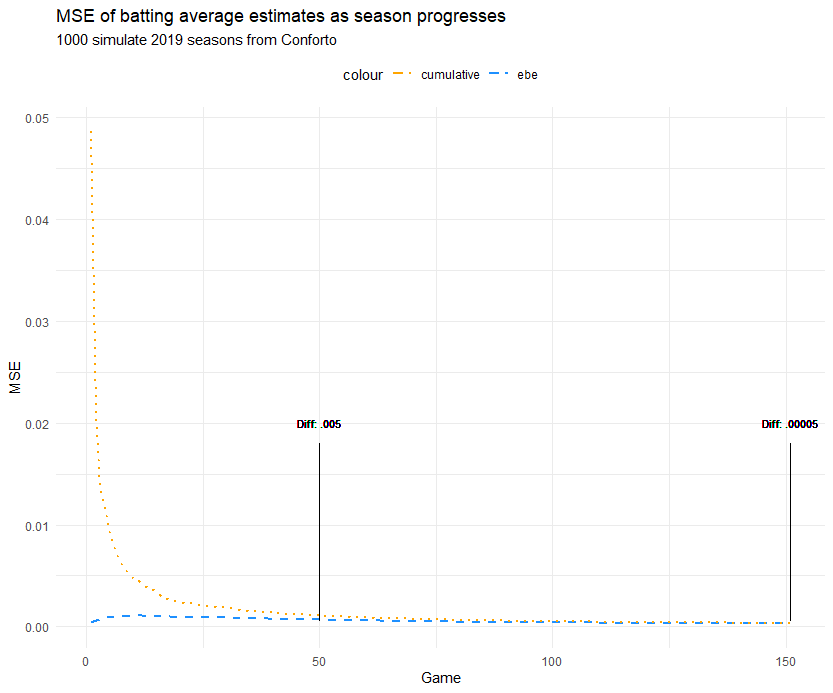
\includegraphics[width=.8\linewidth]{mse_2019}
\end{minipage}
\begin{minipage}{.5\textwidth}
	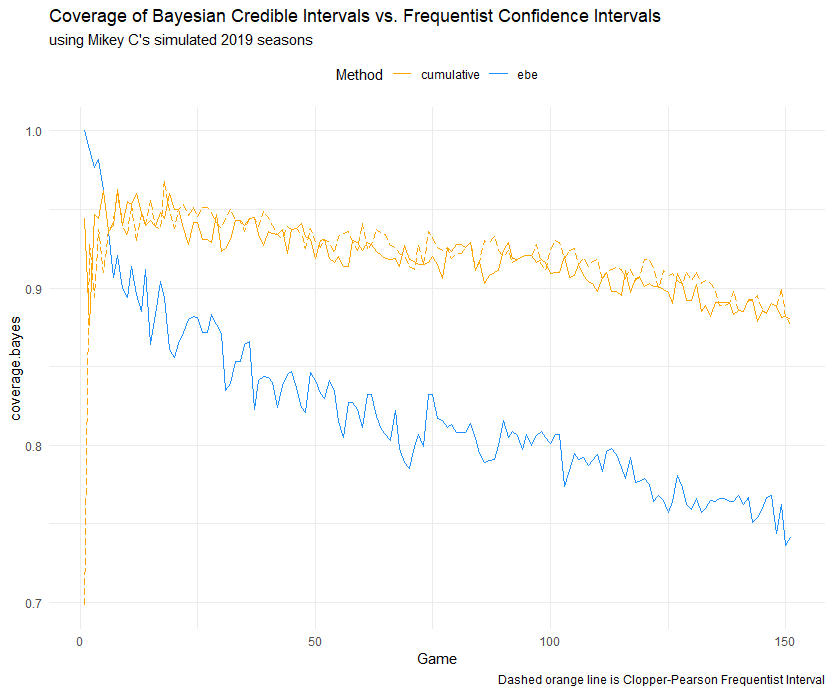
\includegraphics[width=.8\linewidth]{coverages_2019}
\end{minipage}

We see that the MSE for the Bayesian interval is lower than the regular frequentist estimate, however the gap between the estimates diminishes quickly.
In our simulation, by game 50 in the season there was only negligible difference in MSE.

The Bayesian intervals are usually narrower than the frequentist intervals, which also manifests itself in a lower coverage of $p$.
As the season continues, the Bayesian credible interval's coverage decreases until by the end of the season it only covered $p = .257$ roughly 75\% of the time.
However, as \ref{fig:intervals_2019} shows us, neither Bayesian or frequentist intervals are that practical since their intervals are too wide to say much of value about a player's individual hit probability.

\subsection{$p$ changes between simulated seasons}
For this scenario, at the start of each simulated season we will draw random a $p$ from a Beta(45.173, 117.316) distribution, our Beta shifted distribution for Michael Conforto based at a batting average of .279.
The prior mean will be a shifted Beta with mean equal to Conforto's 2016 performance of .220.

The results of our last simulation showed narrow Bayesian credible intervals, so we might want to investigate the distribution of the posterior parameters when the season is completed.
We can then plot $\alpha$ and $\beta$ for all 1000 simulated posterior distributions.

\begin{minipage}{.5\textwidth}
	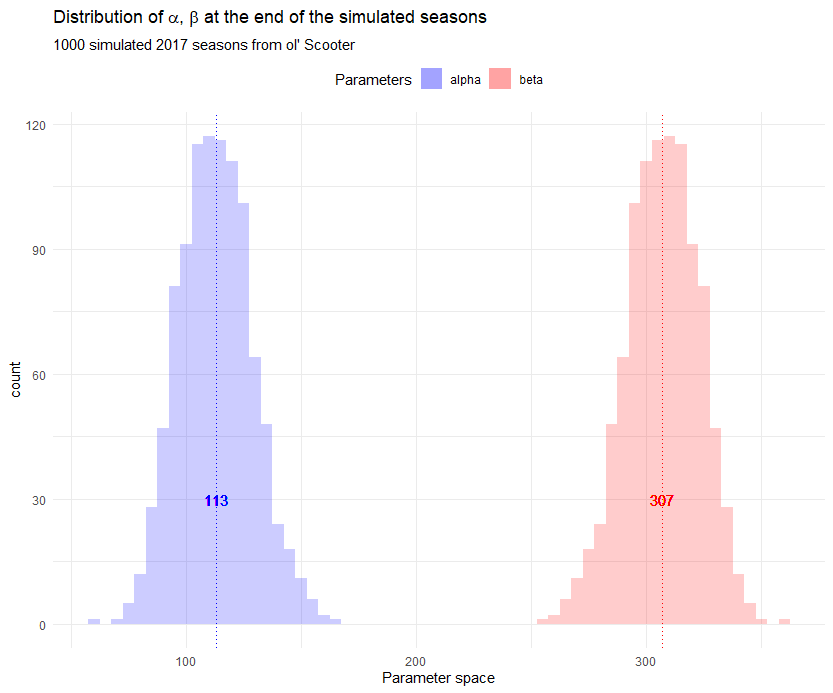
\includegraphics[width=.8\textwidth]{posts_2017}
\end{minipage}
\begin{minipage}{.5\textwidth}
	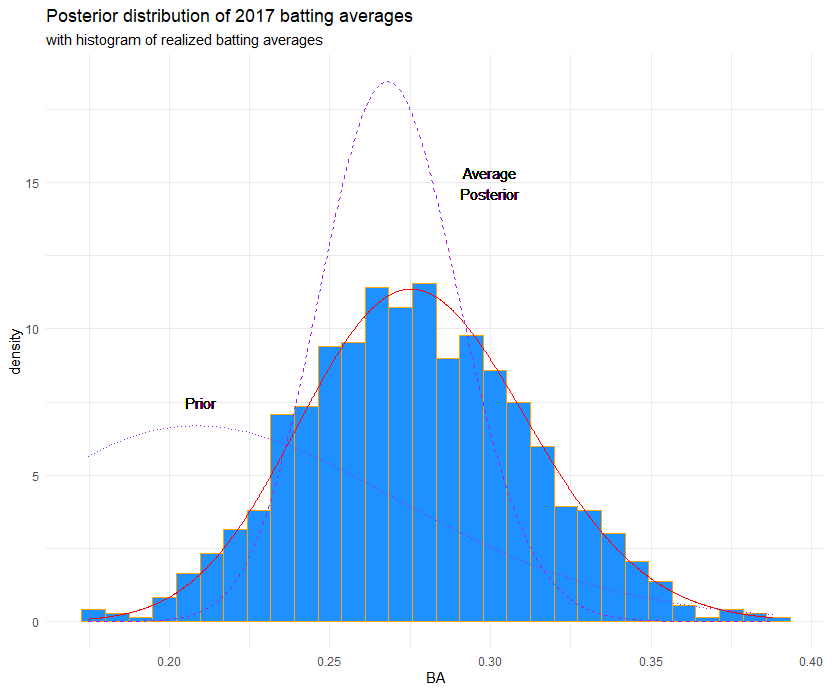
\includegraphics[width=.8\textwidth]{dists_2017}
\end{minipage}

The $\alpha$ and $\beta$ parameters at the end of the season have rougly bell shaped posterior distributions which are centered at 113 and 307 respectively.
Plotting a \texttt{Beta(113, 307)} curve against the histogram of simulated $p$'s, we see that on average the posterior distribution is significantly narrower than the distribution from which $p$ was drawn.
As $\alpha$ and $\beta$ grow, the posterior distribution grows narrower around the mean.
This explains that while the Bayesian estimate was usually accurate, the credible interval has less coverage than we would expect.
In \ref{fig:coverages_2017}, we see a similar story to our first simulation although this time the frequentist interval maintains it 95\% coverage. 

\begin{figure}[ht]
	\centering
	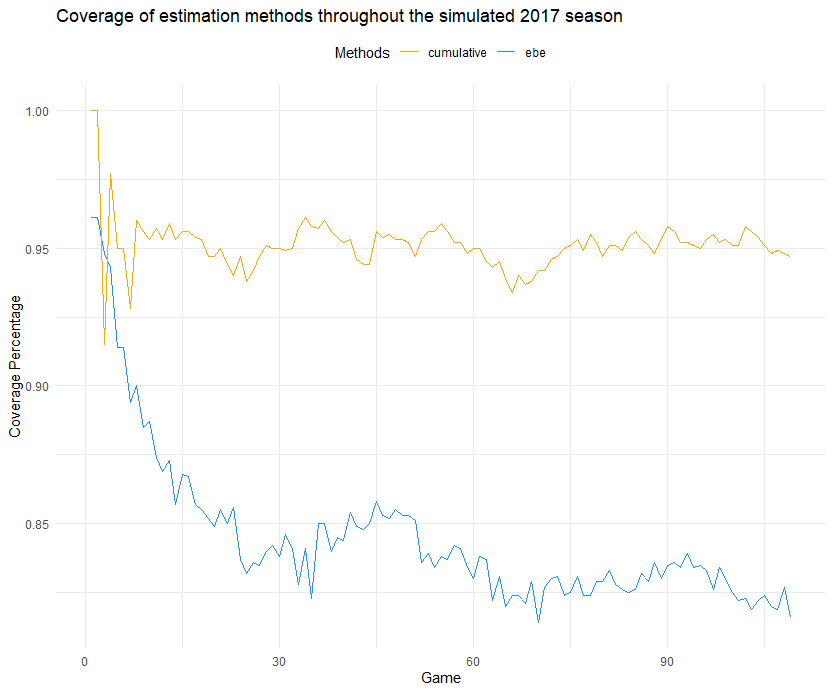
\includegraphics[width=.5\textwidth]{coverages_2017}
	\caption{\label{fig:coverages_2017} Coverage of credible and confidence intervals plotted for the 2017 simulated seasons} 
\end{figure}

\subsection{$p$ changes every game}
A more realistic probability model would be if instead of having a single $p$ for an entire season, what if $p$ was changed every day?
This would more accurately simulate Michael Conforto playing at different ballparks, against different pitchers, etc. and lower MSE here would indicate a $\hat{p}$ estimate which is more practically robust.
Again we sample random $p$ from Beta(45.173, 117.316), but this time $p$ is a vector of probabilities to use over a simulated season instead of a single value.

\begin{minipage}{.5\textwidth}
	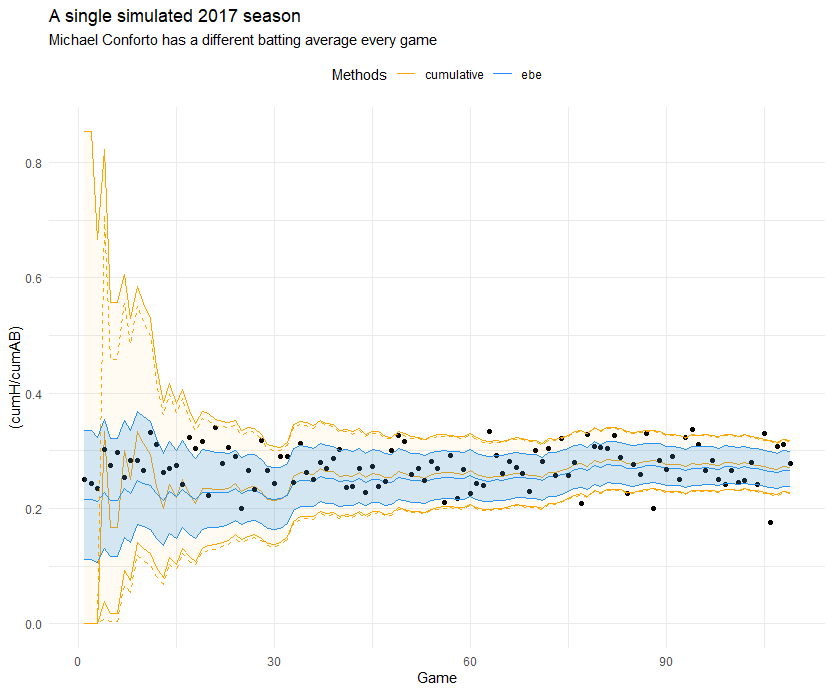
\includegraphics[width=.95\textwidth]{manyp_2017}
\end{minipage}
\begin{minipage}{.5\textwidth}
	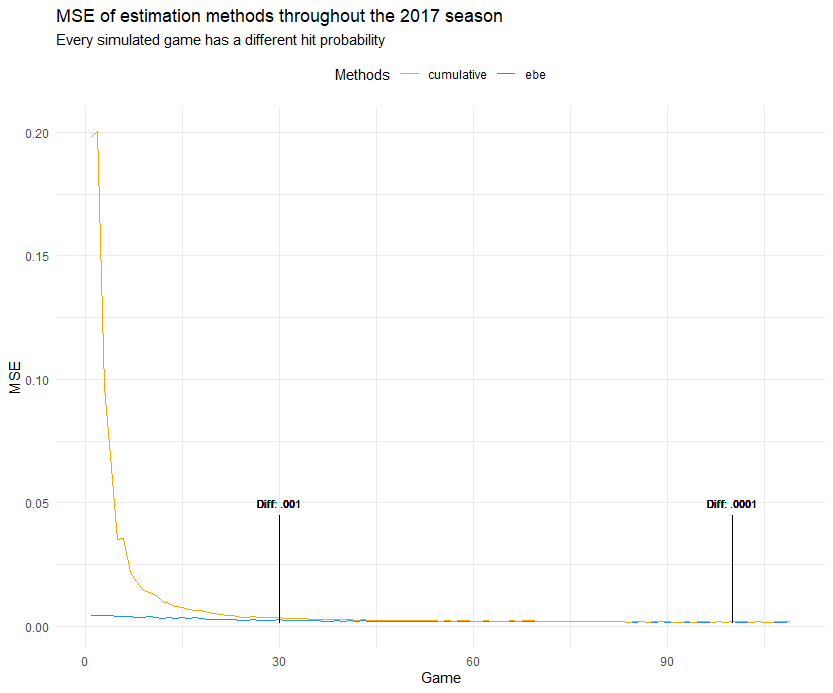
\includegraphics[width=.95\textwidth]{manyp_mse}
\end{minipage}

In the above figures, the right plot shows one such simulated season where the black dots represent $p$ for that given game.
The left figure shows the difference in MSE between the Bayesian and frequentist estimates.
The Bayesian estimate again has a lower MSE than the frequentist estimate, however, this advantage diminishes quickly and is negligible by game 30 in the season.
The interval coverage was also calculated but was very similar to the coverage plots in the other two simulations and therefore are excluded.

\section{Conclusion}
Empirical Bayesian estimation with a prior based on the last season's performance had a lower MSE in all simulations and all time points.
This held true even in scenarios where $p$ varied even between games.
However, this advantage in MSE only practically significant in the beginning of the season.
By the midpoint, the MSE benefit is very minimal.
However, the Bayesian estimate can still fill the niche in early season player evaluation for an estimate of hit probability with relatively low bias and variance.

Finally, while Bayesian credible intervals are narrower than frequentist intervals owing to the lower variance of the posterior distribution as $\alpha$ and $\beta$ grow, both Bayesian and Frequentist intervals are too wide to be of much practical use (average width being around .1 for Bayesian intervals which in a baseball context is enormous).

\section{Code}
All data and code for this project is publicly available at \texttt{www.github.com/njjms/bayesball}

\section{References}
\printbibliography

\end{document}
